\documentclass[conference]{IEEEtran}
\usepackage{amsmath, amssymb}
\usepackage{graphicx}
\usepackage{booktabs}
\usepackage{hyperref}

% 図の検索パスを figs/ に通す
\graphicspath{{figs/}}

\title{SystemDK with AITL: Physics-Aware Runtime DTCO via PID, FSM, and LLM Integration}

\author{
  \IEEEauthorblockN{Shinichi Samizo}
  \IEEEauthorblockA{Independent Semiconductor Researcher \\
  Email: shin3t72@gmail.com}
}

\begin{document}
\maketitle

\begin{abstract}
This paper presents SystemDK with AITL, a framework that extends conventional Design-Technology Co-Optimization (DTCO) by embedding control-theoretic loops directly into EDA flows. Compact PID controllers and FSM supervisors stabilize runtime variations (RC delay, thermal coupling, EMI/EMC disturbances). Future extensions (AITL Next) integrate LLM analyzers for adaptive PID retuning and FSM rule regeneration. The framework incorporates FEM analysis and S-parameter measurements into synthesis, P\&R, and STA, ensuring physics-aware closure. Simulations demonstrate order-of-magnitude improvements in timing stability, thermal robustness, and jitter suppression.
\end{abstract}

\section{Introduction}
Scaling to sub-2nm nodes and CFET integration introduces critical runtime effects:
\begin{itemize}
  \item RC delay variation due to interconnect scaling,
  \item Vertical thermal coupling in 3D-ICs,
  \item Stress-induced $V_{th}$ shifts,
  \item EMI/EMC noise degrading jitter and reliability.
\end{itemize}
Traditional DTCO applies static guardbands, leading to inefficiency. SystemDK with AITL proposes embedding runtime control (PID+FSM) and, in the future, LLM-based adaptation.

\section{Proposed Framework}
\subsection{AITL Base}
PID compensates delay/thermal/voltage variations; FSM supervises modes and safety thresholds.
\subsection{AITL Next}
LLM (lightweight, future) analyzes EDA logs, retunes PID gains $(K_p, K_i, K_d)$, and regenerates FSM rules.

\begin{figure}[h]
  \centering
  \includegraphics[width=0.48\textwidth]{system_overview.png}
  \caption{System overview: Control layer (PID+FSM), EDA flow, FEM/S-parameter integration, actuators, and LLM (Next).}
\end{figure}

\section{Analytical Models and EDA Mapping}
\subsection{RC Delay Model}
\[
t_{pd}(T,\sigma,f) = R_0 \cdot (1+\alpha_T (T-T_0)+\alpha_\sigma \sigma)\,C(f)+\Delta_{EMI}(f)
\]
Mapped to STA path delay constraints.

\subsection{Thermal Coupling}
\[
C_{th}\frac{dT}{dt} + \frac{T-T_{amb}}{R_{th}} = P_{chip}(t)
\]
Mapped to P\&R thermal placement constraints.

\subsection{Stress-Induced Vth Shift}
\[
\Delta V_{th}(\sigma)=\kappa \cdot \sigma
\]
Mapped to PDK/SPICE parameter updates.

\subsection{EMI Injection}
\[
v_{emi}(t)=A\sin(2\pi f_{emi} t)
\]
Mapped to SI/EMC jitter constraints.

\section{Simulation Results with EDA Implications}
\subsection{RC Delay Compensation}
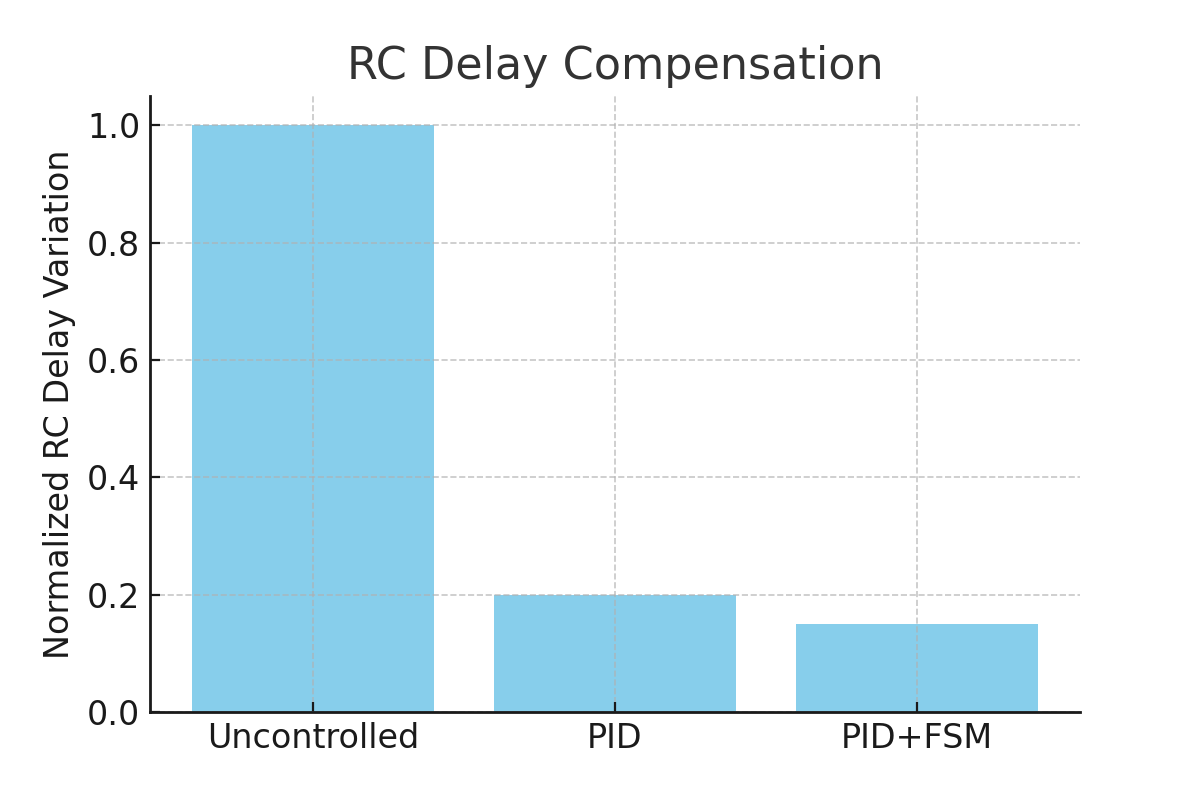
\includegraphics[width=0.45\textwidth]{sim_delay_rc.png}

\subsection{Thermal Response Control}
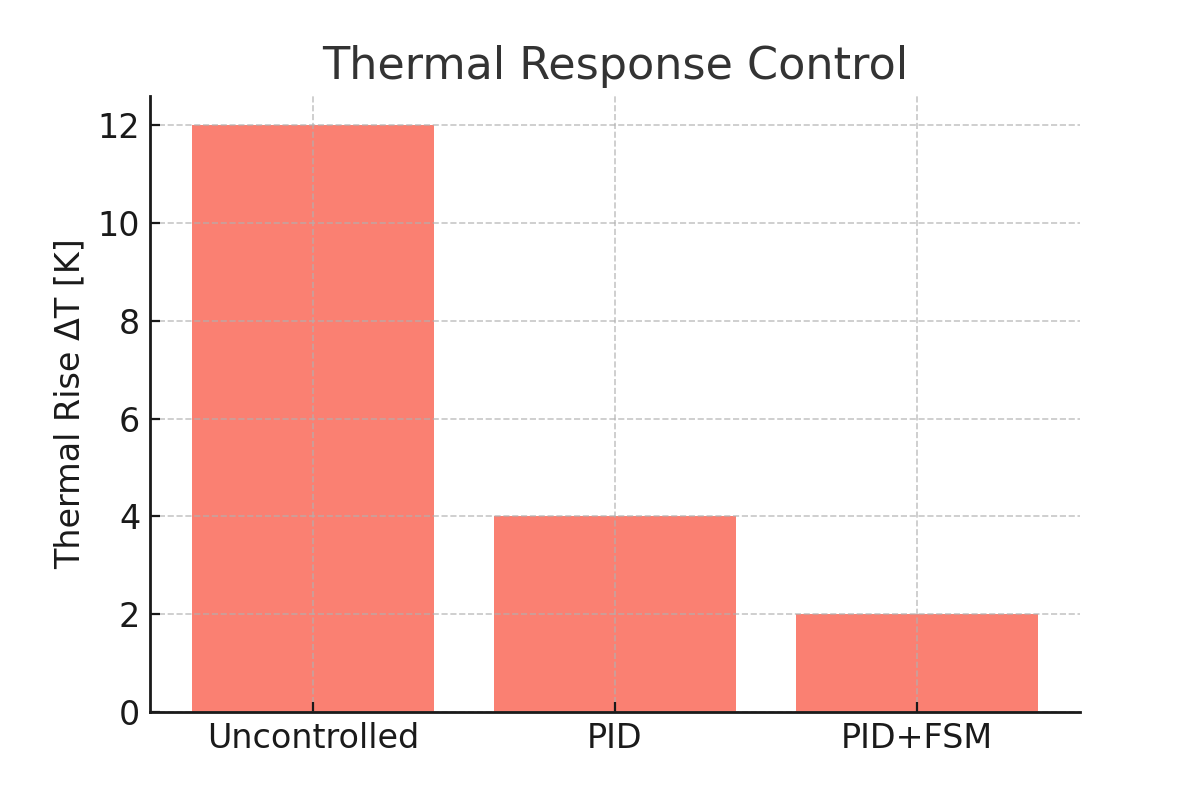
\includegraphics[width=0.45\textwidth]{sim_thermal_response.png}

\subsection{EMI Jitter Suppression}
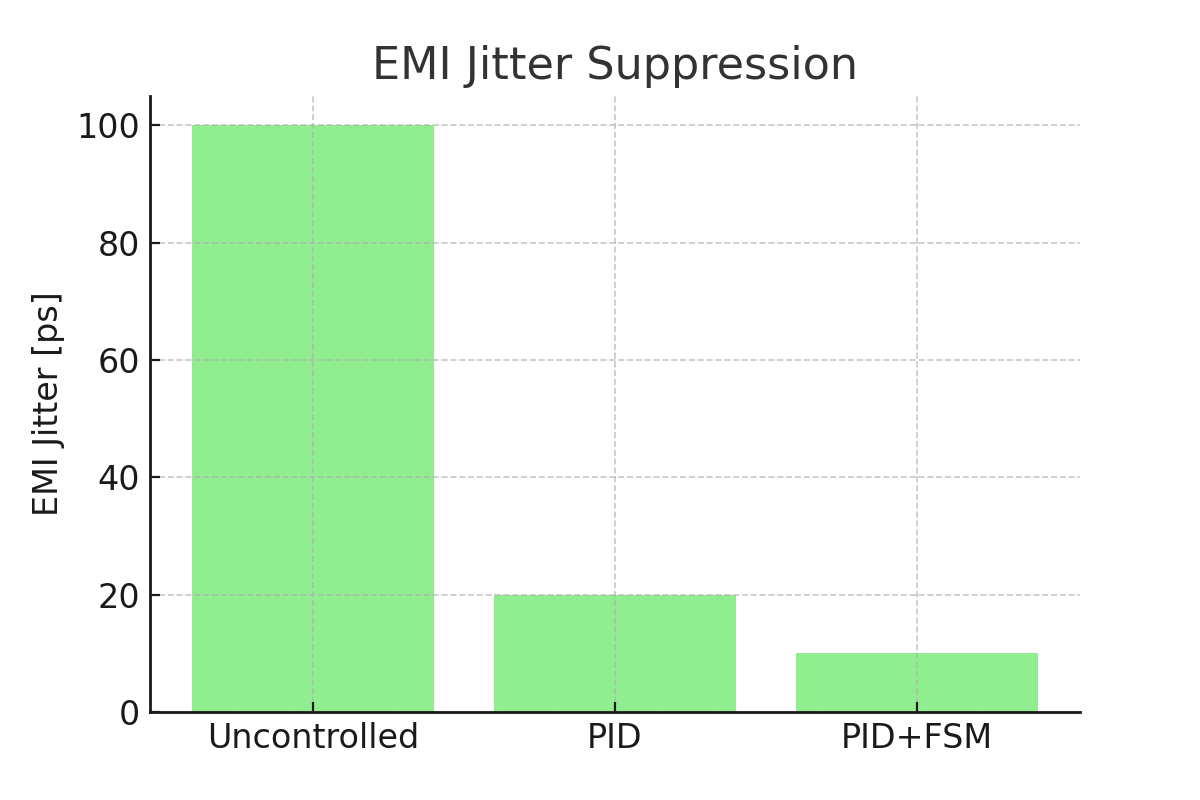
\includegraphics[width=0.45\textwidth]{sim_emi_jitter.png}

\subsection{FEM Analysis}
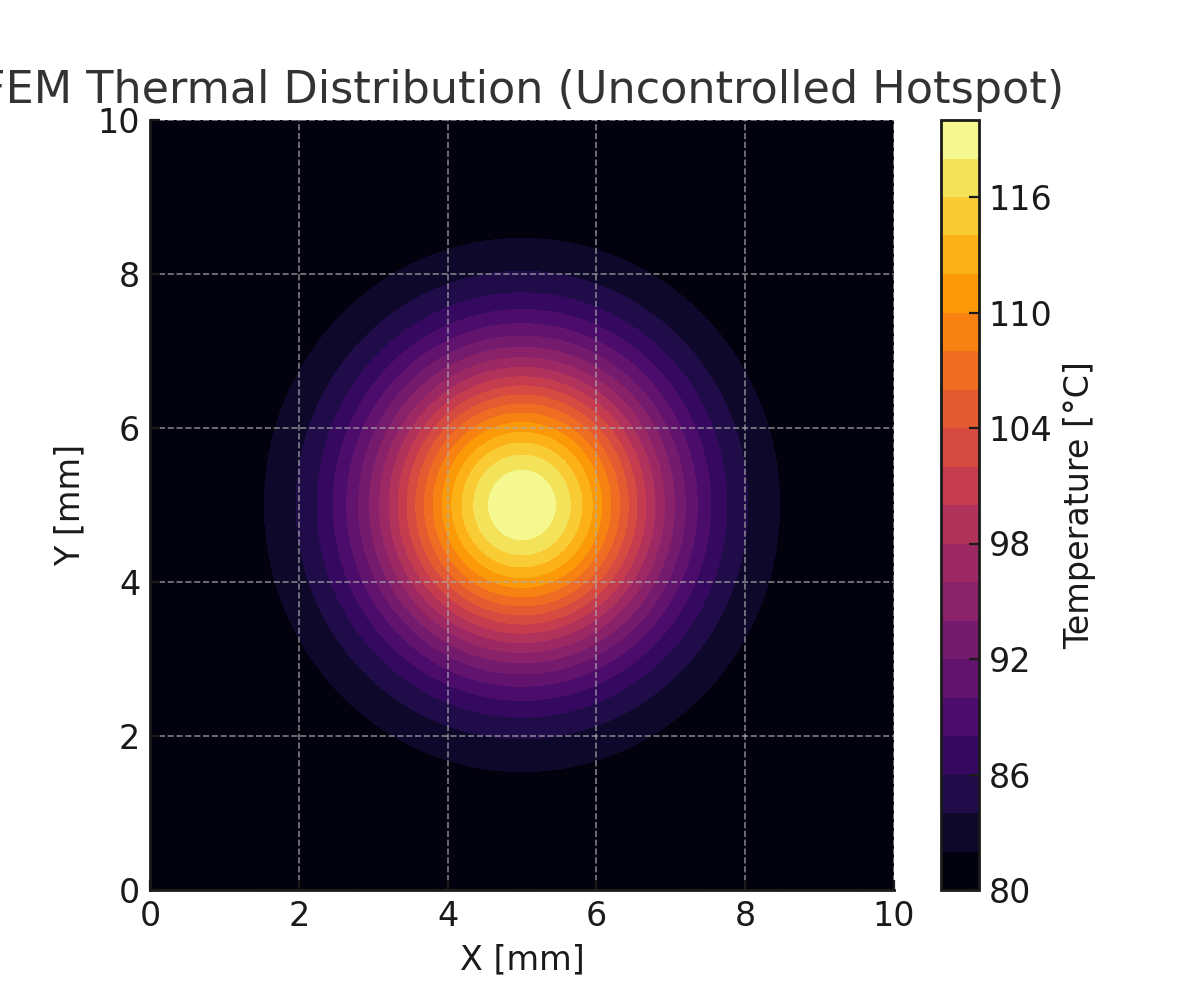
\includegraphics[width=0.45\textwidth]{fem_thermal_map.png}
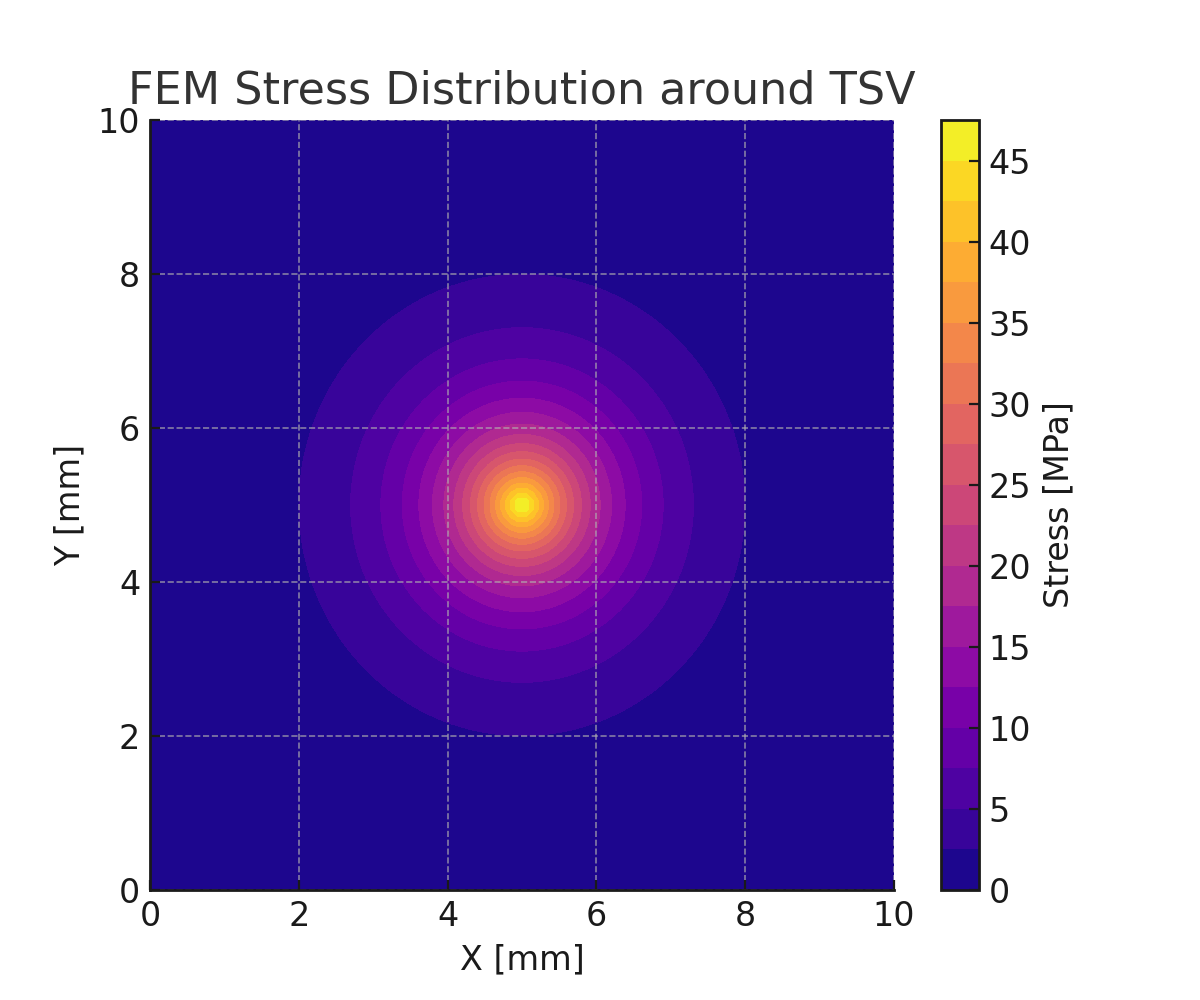
\includegraphics[width=0.45\textwidth]{fem_stress_map.png}

\subsection{S-Parameter Analysis}
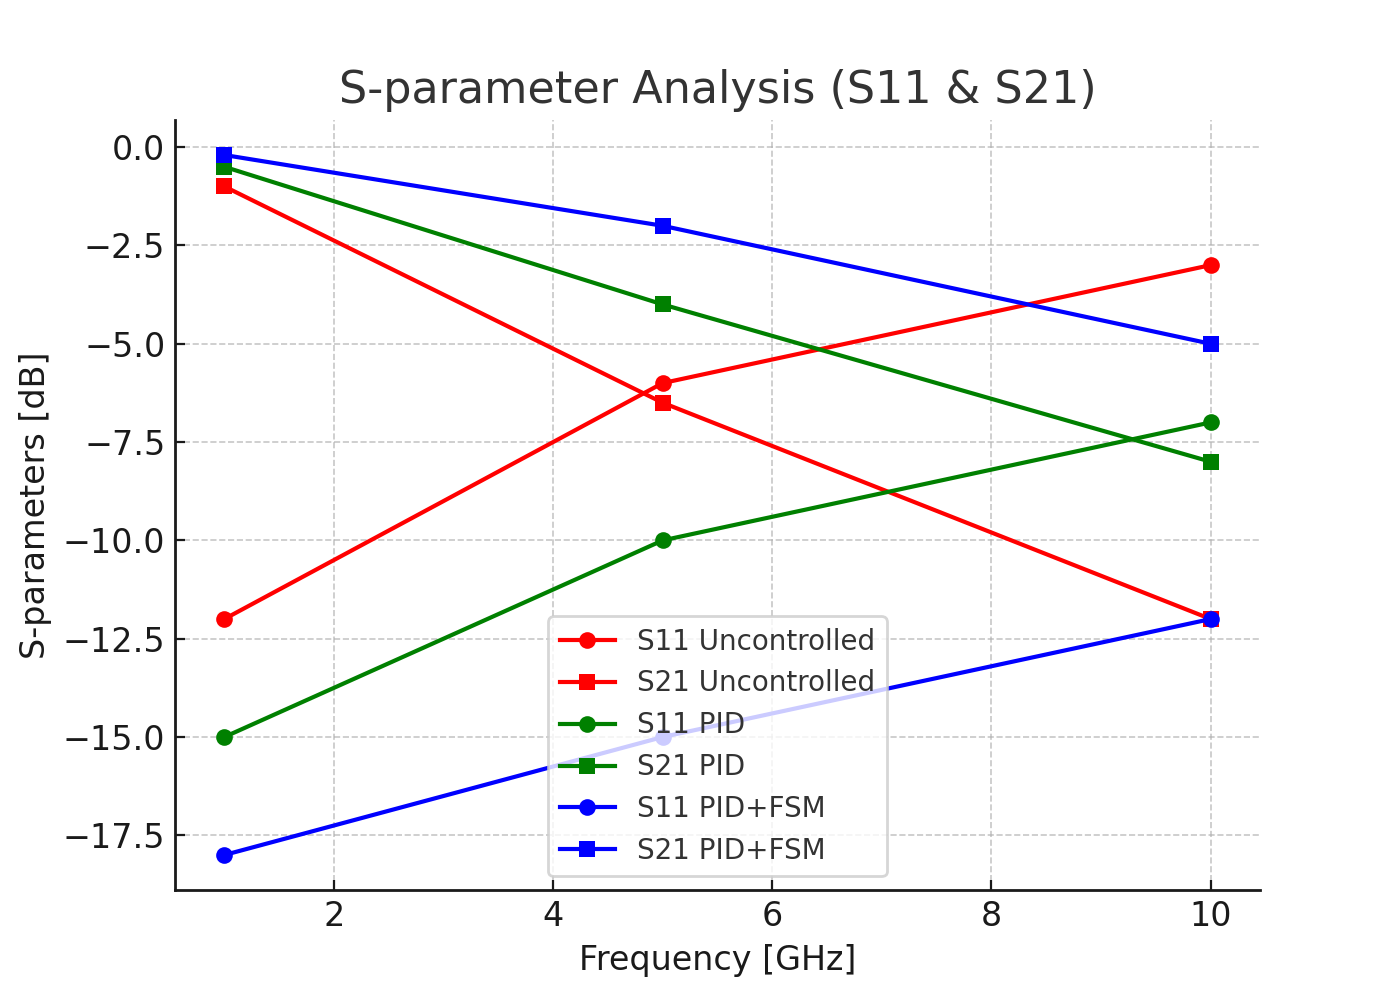
\includegraphics[width=0.48\textwidth]{sparam_s11s21.png}

\section{Implementation PoC}
RTL excerpt (PID controller), FSM transitions, and YAML configuration were implemented in Verilog and integrated with APB/AXI-Lite CSRs.

\section{Discussion}
\begin{itemize}
  \item Guardbands $\to$ adaptive loops,
  \item Static sign-off $\to$ dynamic runtime closure,
  \item Reliability $\to$ cross-domain resilience (delay, thermal, stress, EMI).
\end{itemize}

\section{Conclusion and Future Work}
AITL Base (PID+FSM) establishes runtime stabilization.
AITL Next will integrate lightweight LLM models for real-time EDA log analysis and control redesign.
Industrial relevance: prototype chips, EDA tool collaboration, and AI-driven DTCO.

\bibliographystyle{IEEEtran}
% ← ここを bib の実ファイル名に合わせて修正
\bibliography{systemdk_aitl2025}

\end{document}
